\section{BIP38: 基于口令保护私钥}

BIP38提出了基于口令(Passphrase/Password)对私钥进行加密保护的方案.
该方案只考虑了针对私钥的机密性保护,而没有考虑提供完整性保护(从密码学角度来讲不算是最佳实践),
因此其主要针对纸钱包(Paper Wallet)等私钥密文不容易遭受篡改的应用场景.
BIP38中给出了两种加密私钥的方法,其中一种方法使用了EC乘法操作,
另一种没有使用EC乘法操作.两种方法实现的功能有很大的区别.
方便起见,后续我们用方法一指代没有使用EC乘法操作的加密方法,用方法二指代使用了EC乘法操作的加密方法.

未使用EC乘法操作的方法一中, 对于已经产生的私钥, 使用用户设置的口令对私钥进行加密.
加密后的密文与口令在解密私钥时缺一不可.由于两者可以独立管理,可以提高私钥的安全性.

使用了EC乘法操作的方法二中, 用户首先会生成一个中间口令码(Intermediate Passphrase Code),
%(包含一个由passphrase单向生成的椭圆曲线群上的点,以及用户产生的salt),
并将其传输给一个第三方.
%(由于该方案针对的场景主要是纸钱包,这里的第三方通常是一个printer),
第三方可以为用户生成新的地址,并将新地址和计算地址对应的私钥所必须的信息发给用户
%并对恢复该地址对应私钥的必要信息加密后展示给用户.
用户拿到前述信息后结合口令,即可算出新地址对应的私钥.
这种方式允许用户将生成新地址的工作委托给无需可信的第三方来做,但同时保证只有知道口令和密文的人才能计算出对应私钥.

%BIP38同时给出了对应于两种方法的密文数据编码方式,虽然格式不同,但长度都为39个字节.
%方法一中最终的密文数据为以下字节序列\textsf{Base58Check}编码:
%$$0x01 || 0x42 || flagbyte || addrhash || encryptedhalf_1 || encryptedhalf_2.$$
%方法二中最终的密文数据为以下字节序列的\textsf{Base58Check}编码:
%$$0x01 || 0x43 || flagbyte || addrhash || ownerentropy || encryptedhalf_1 || encryptedhalf_2.$$
%
%\begin{itemize}
%\item 对于不使用EC乘法的,最终的数据由对$0x01 \ 0x42+ flagbyte+ addrhash+ encryptedhalf1 + encryptedhalf2$
%进行Base58Check编码后的数据构成.而对于使用EC乘法的,加密保护后的私钥数据由
%$0x01 \ 0x43+ flagbyte+ addrhash+ ownerentropy+ encryptedhalf1 \  + encryptedhalf2$
% 进行Base58Check编码后的数据构成(具体含义会在后面详细介绍).
%
%\item $0x01\ 0x42/43$是为了使经过Base58Check编码后的结果以$6P$开头,
%6代表了"a private key that needs something else to be usable",P代表了上一句中的"something is a passphrase".
%
%\item flagbyte为1字节,最高两位用来区分是否使用EC乘法:
%11表示不使用EC乘法,反之设置为00.$0x20$用来表示私钥转换成比特币地址时使用的是压缩公钥的格式.
%$0x40$用来表示在使用EC乘法时,同时也使用了lot+sequence,这两个数字的作用会在后面说明.$0x10,0x08$予以保留.
%
%\item Addrhash为对比特币地址进行两次SHA256操作后,取前四个字节的结果.
%\end{itemize}

\subsection{不使用EC乘法的加密方法一}

该方法对已有私钥$k$进行加密,加密过程分为两步:用Scrypt算法从口令t派生AES算法加密所需密钥;使用AES算法对私钥信息进行加密.
记该私钥对应的Bitcoin地址为$address$, 按照以下Algorithm~\ref{algo-m1}~展示的步骤进行.

\begin{algorithm}[h]\footnotesize
\caption{不使用EC乘法的加密方法一}\label{algo-m1}
\begin{algorithmic}[1]
	    	\STATE 计算地址哈希值 $addresshash = \textsf{SHA256}(\textsf{SHA256}(address))[0,1,2,3]$
		\STATE 用Scrypt根据口令等派生32字节值$v=v_1||v_2, v_1 = v[0,\cdots, 31], v_2= [32,\cdots,63]$
		\STATE 计算$ek_1 = \textsf{AES256Encrypt}(block = k[0...15] \oplus v_1[0,\cdots,15], key = v_2)$
		\STATE 计算$ek_2 = \textsf{AES256Encrypt}(block = k[16...31] \oplus v_1[16...31], key = v_2)$
		\STATE 密文为$0x01 || 0x42 || flagbyte || addrhash || ek_1 || ek_2$的\textsf{Base58CheckEncode}
\end{algorithmic}
\end{algorithm}


%\begin{enumerate}
%\item 计算地址哈希值 $addresshash = \textsf{SHA256}(\textsf{SHA256}(address))[0,1,2,3]$
%\item 用Scrypt根据口令等派生32字节值$v=v_1||v_2, v_1 = v[0,\cdots, 31], v_2= [32,\cdots,63]$
%\item 计算$ek_1 = \textsf{AES256Encrypt}(block = k[0...15] \oplus v_1[0,\cdots,15], key = v_2)$
%\item 计算$ek_2 = \textsf{AES256Encrypt}(block = k[16...31] \oplus v_1[16...31], key = v_2)$
%\item 密文为$0x01 || 0x42 || flagbyte || addrhash || ek_1 || ek_2$的\textsf{Base58Check}编码
%\end{enumerate}


\begin{figure}[h]
\centering
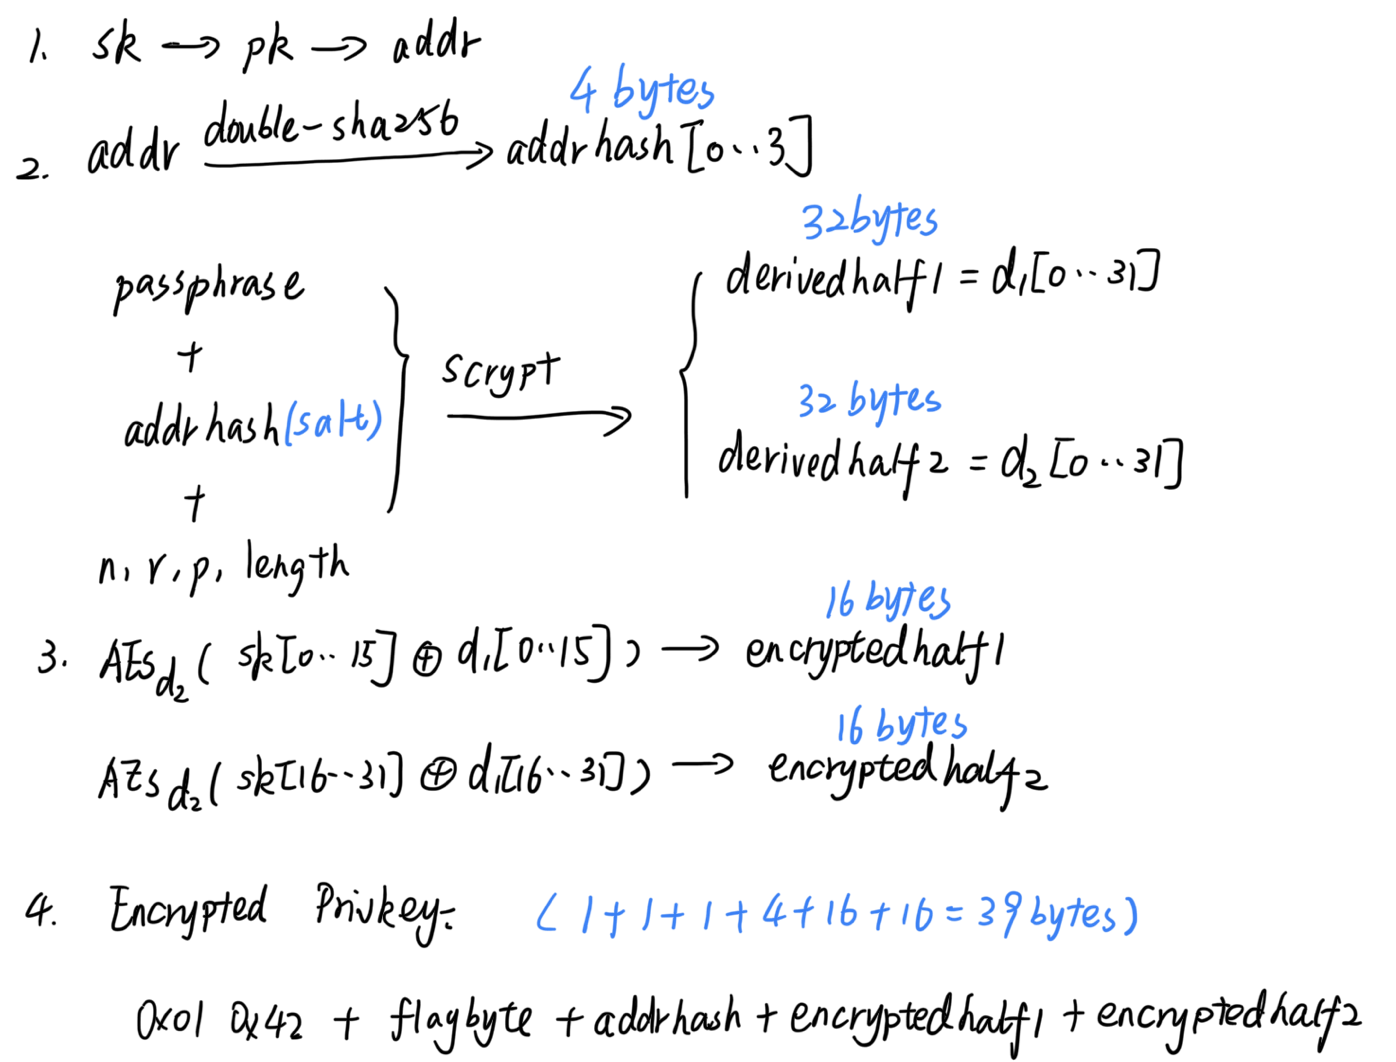
\includegraphics[width=.7\textwidth]{./no-ec.png}
\caption{不使用EC乘法的加密方法一: 加密过程}\label{fig-m1-enc}
\end{figure}

在使用Scrypt派生密钥时, Scrypt参数中passphrase值为用UTF-8编码
并用NFC (Unicode Normalization Form C)正则化后的口令,
salt设置为$addresshash$,也即$ \textsf{SHA256}(\textsf{SHA256}(address))$的前4个字节, 
该字段无需保密,目的是为了引入更多的熵值,以增加攻击者进行暴力破解时的搜索空间.
$n, r, p$的值为系统设置参数,并且$n=16384, r=8, p=8, length=64$.
最终的密文为39个字节,参见Figure~\ref{fig-m1-enc}.
其中$flagbyte$为1个字节,最高两位用来区分是否使用EC乘法:
$flagbyte_{7,6}=11$表示不使用EC乘法,
$flagbyte_{7,6}=00$表示使用了EC乘法.
比特$flagbyte_{5}=1$表示使用比特币地址是根据压缩形式的公钥计算而来的,
注意Bitcoin中同一个私钥可以有两种比特币地址,分别对应压缩形式公钥和不压缩形式公钥.
$flagbyte_{3}=1$表示在使用EC乘法加密时还使用了lot+sequence字段,这两个字段的作用会在后面说明.
其余比特位保留.
[todo这里有问题 关于flagbyte]


%\begin{algorithm}[h]\footnotesize
%\caption{Encryption}\label{encryption without ec multiply}
%  	\begin{algorithmic}[1]
%	    \STATE 计算Bitcoin地址(ASCII), 计算addresshash,也即地址哈希值$\textsf{SHA256(SHA256())}$的前4个字节
%		\STATE 用scrypt从口令派生密钥
%	⁃	
%		\STATE 参数: passphrase 是用UTF-8编码并用NFC (Unicode Normalization Form C)正则化后的值. 
%		salt 是之前计算的addresshash, $n=16384, r=8, p=8, length=64 $(n, r, p are provisional and subject to consensus)  
%		\STATE Let's split the resulting 64 bytes in half, and call them derivedhalf1 and derivedhalf2
%		\STATE Do $encryptedhalf1 = \textsf{AES256Encrypt}(block = bitcoinprivkey[0...15] \oplus derivedhalf1[0...15], key = derivedhalf2)$,
%		\STATE Do $encryptedhalf2 = AES256Encrypt(block = bitcoinprivkey[16...31] \oplus derivedhalf1[16...31], key = derivedhalf2)$, 
%		\STATE The encrypted private key is the Base58Check-encoded concatenation of the following, which totals 39 bytes without Base58 %checksum:$0x01$ $0x42 + flagbyte + salt + encryptedhalf1 + encryptedhalf2$
%    \end{algorithmic}
%\end{algorithm}

解密过程首先根据用户掌握的passphrase计算出AES的解密密钥,随后对密文解密,
首先也需要通过Scrypt计算$v_1, v_2$, 然后利用\textsf{AES256Encrypt}解密得到私钥的值,
通过私钥根据$flagbyte$中的信息派生Bitcoin地址,并进一步计算$addresshash$并与密文中的该字段进行对比.
如果不匹配则报告输入的口令错误. 加密和解密的PoC代码实现参见Listing~\ref{lst-m1},
执行结果参见Listing~\ref{lst-m1res}.


%\begin{algorithm}[h]\footnotesize
%\caption{Decryption}
%  	\begin{algorithmic}[1]
%	    \STATE Collect encrypted private key and passphrase from user.  
%		\STATE Derive derivedhalf1 and derivedhalf2 by passing the passphrase and addresshash into scrypt function.
%		\STATE Decrypt encryptedhalf1 and encryptedhalf2 using AES256Decrypt, merge them to form the encrypted private key. 
%		\STATE Convert that private key into a Bitcoin address, honoring the compression preference specified in flagbyte of the encrypted %key record.
%		\STATE Hash the Bitcoin address, and verify that addresshash from the encrypted private key record matches the hash. If not, report %that the passphrase entry was incorrect.  
%    \end{algorithmic}
%\end{algorithm}

\begin{lstlisting}[language=python, caption = 不使用EC乘法的加解密过程示例, label=lst-m1]

import hashlib 
import secrets
from Crypto.Cipher import AES
import base58check
import scrypt
from bitcoinlib.keys import *
import ecdsa
from ecdsa.curves import SECP256k1
from ecdsa.ecdsa import int_to_string, string_to_int

# parameter for Scrypt function
SCRYPT_N=16384
SCRYPT_R=8
SCRYPT_P=8

def b58check(data):
	# return base58 encoding of data with checksum
	checksum=hashlib.sha256(data).digest()
	checksum=hashlib.sha256(checksum).digest()
	data+=checksum[:4]
	return base58check.b58encode(data)

def enc_without_ec_multi(privkey,address,passphrase,compressed):
	# compute addrhash of corresponding address to known private key
	addrhash=hashlib.sha256(address).digest()
	addrhash=hashlib.sha256(addrhash).digest()
	addrhash=addrhash[:4]
	# derive encryption key for AES
	passphrase=passphrase.decode('utf-8')
	d=scrypt.hash(passphrase,addrhash,SCRYPT_N,SCRYPT_R,SCRYPT_P,64)
	derivedhalf1=d[:32]
	derivedhalf2=d[32:64]
	# encryption process
	m1=[a^b for a,b in zip(privkey[:16],derivedhalf1[:16])]
	m2=[a^b for a,b in zip(privkey[16:32],derivedhalf1[16:32])]
	e1=AES.new(derivedhalf2).encrypt(bytes(m1))
	e2=AES.new(derivedhalf2).encrypt(bytes(m2))
   # pack encryption data
	flagbyte=b'\xe0' if compressed==1 else b'\xC0'
	res=b'\x01\x42'+flagbyte+addrhash+e1+e2
	return b58check(res)
	
def dec_without_ec_multi(encrypted_privkey,passphrase):
	# unpack data 
	data=base58check.b58decode(encrypted_privkey)
	addrhash_v=data[3:7]
	passphrase=passphrase.decode('utf-8')
	# derive decryption key for AES
	d=scrypt.hash(passphrase,addrhash_v,SCRYPT_N,SCRYPT_R,SCRYPT_P,64)
	derivedhalf1=d[:32]
	derivedhalf2=d[32:64]
	# decryption process
	m1=AES.new(derivedhalf2).decrypt(data[7:23])
	m2=AES.new(derivedhalf2).decrypt(data[23:39])
	privkey1=bytes([a^b for a,b in zip(m1,derivedhalf1[:16])])
	privkey2=bytes([a^b for a,b in zip(m2,derivedhalf1[16:32])])
	privkey=privkey1+privkey2
	# verify whether addrhash is correct
	k=Key(privkey)
	addr=k.address_uncompressed() if data[2]==0xC0 else k.address()
	addrhash=hashlib.sha256(addr.encode('ascii')).digest()
	addrhash=hashlib.sha256(addrhash).digest()
	if addrhash!=addrhash_v:
		assert("address is not valid!")
	else:
		return privkey1+privkey2
\end{lstlisting}


\begin{lstlisting}[language=bash, caption = Listing~\ref{lst-m1}~的执行结果示例, label=lst-m1res]
Encryption with no EC multiplication:
Privkey is : b'\xcb\xf4\xb9\xf7\x04p\x85k\xb4\xf4\x0f\x80\xb8~\xdb\x90\x86Y\x97\xff\xeem\xf3\x15\xab\x16mq:\xf43\xa5'
Encrypted private key is : b'6PRVWUbkzzsbcVac2qwfssoUJAN1Xhrg6bNk8J7Nzm5H7kxEbn2Nh2ZoGg'

Decryption with no EC multiplication:
Decryption succeed!
Private key is  b'\xcb\xf4\xb9\xf7\x04p\x85k\xb4\xf4\x0f\x80\xb8~\xdb\x90\x86Y\x97\xff\xeem\xf3\x15\xab\x16mq:\xf43\xa5'
\end{lstlisting}


\subsection{使用EC乘法的加密方法二}

该方法利用了EC 乘法的同态性质,主要思想类似于一个基于椭圆曲线的密钥协商方案.
用户事先由口令和熵值等生成一个随机数$x$,并计算对应的椭圆曲线群上的点$P=xG$,将其发给第三方.
随后第三方选择一个随机数$k$与该点进行EC的乘法操作,也即新生成的公钥$P'=kP=(x \cdot k)G$.
随后将$k$加密后发送给用户(加密过程与方法一中类似).
用户收到数据解密后,计算出新私钥$x\cdot k$.
假设用于生成$x$的口令没有泄露,则用户就可以确认新私钥是足够安全的(只有知道口令的人才能计算出新私钥), 
%这一点可以认为是使用该方法生成新的加密私钥所额外带来的一个安全性方面的好处.
方法二主要包括两个阶段:初始化阶段和私钥生成阶段.

初始化阶段主要功能是用户利用口令和熵值计算中间口令码(Intermediate Passphrase Code)并发送给第三方.  
在计算时,用户可以选择性的生成一个20比特的批号(Lot Number)和12比特的序列号(Sequence Number).
在用户向第三方请求大量的加密私钥时,需要检查返回的私钥对应的批号和序列号与用户自己提供的中间口令码中的一致.
4个字节批号和序列号并不是必须的.根据是否使用这两个字段,初始化阶段稍微不同. 
 
 
 在使用批号和序列号时, 按照Algorithm~\ref{algo-m2initwithlnsn}~中的步骤进行初始化. 
 其中第3步中Scrypt输入参数中的passphrase为UTF-8编码的并用NFC形式正则化后的用户口令,
 salt为第1步中生成的$ownersalt$,  $n=16384, r=8, p=8, length=32$.
 第5步中的点的压缩表示形式约束仅限于这一步的计算, 与生成Bitcoin地址时使用的公钥的表示形式无关.
 
\begin{algorithm}[h]\footnotesize
\caption{使用批号和序列号时的初始化阶段}\label{algo-m2initwithlnsn}
  	\begin{algorithmic}[1]
	   	 \STATE 生成4个字节的随机数$ownersalt$
		\STATE 批号和序列号用大端法形式的4字节的整数$lotsequence=lotnumber * 4096 + sequencenumber$
		\STATE  用Scrypt从口令等信息派生32字节密钥$prefactor$
		\STATE 计算$passfactor = \textsf{SHA256}(\textsf{SHA256}(prefactor || ownerentropy))$
		\STATE 计算 $passfactor * G$, 该点的压缩表示形式记为$passpoint$
		\STATE 传送$ownerentropy = ownersalt || lotsequence$以及$passpoint$给第三方
    \end{algorithmic}
\end{algorithm}

 \begin{figure}[h]
\centering
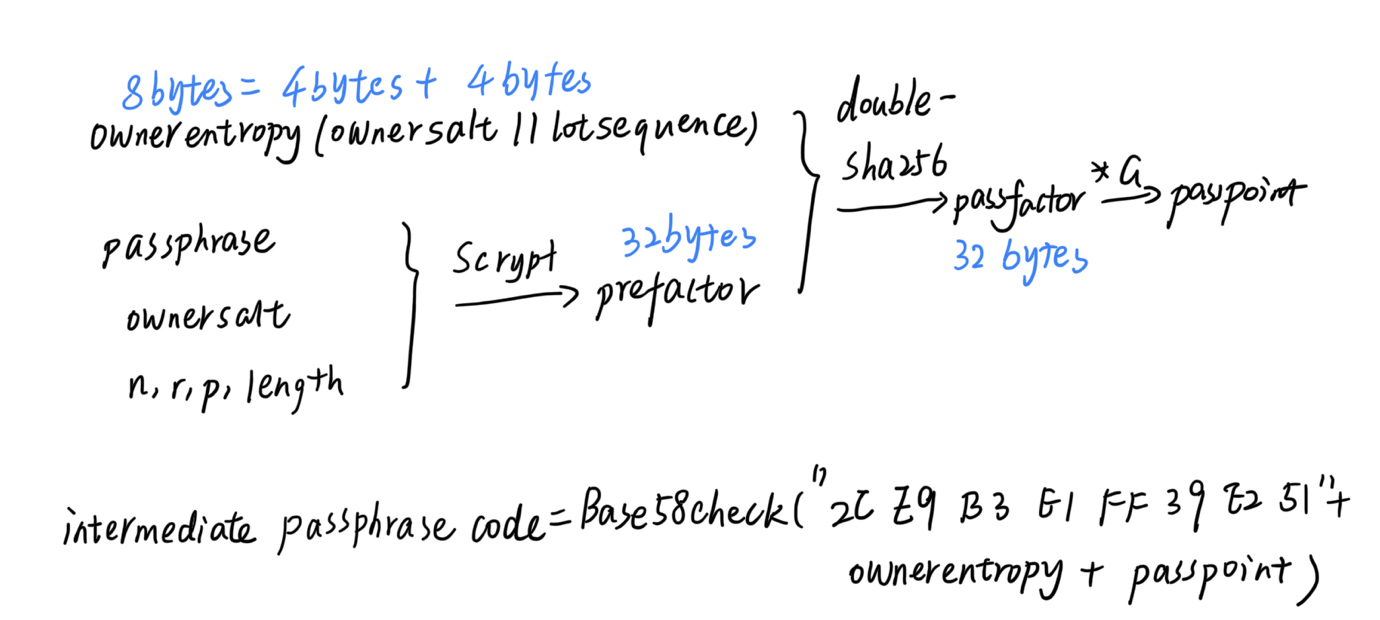
\includegraphics[width=.7\textwidth]{./im-code1.png}
\caption{使用批号和序列号时方法二的初始化过程}\label{fig-m2initwithlnsn}
\end{figure}
 
最后一步中真正发送给第三方的是下面名为\textit{intermediate_passphrase_string}的字符串
(也就是前述的中间口令码):
$$\textsf{Base58CheckEncode}(\textit{2C E9 B3 E1 FF 39 E2 51} || ownerentropy || passpoint)$$
由于魔数(Magic Number) ``2C E9 B3 E1 FF 39 E2 51"的采用,
编码之后的字符串会以``passphrase"开头. 
72个字符的\textit{intermediate_passphrase_string}编码了49个字节的信息以及校验码
49个字节的信息包括8字节的魔数, 8字节的\textit{ownerentropy}以及33字节的\textit{passpoint}.
参见Figure~\ref{fig-m2initwithlnsn}.
 
 
\begin{figure}[h]
\centering
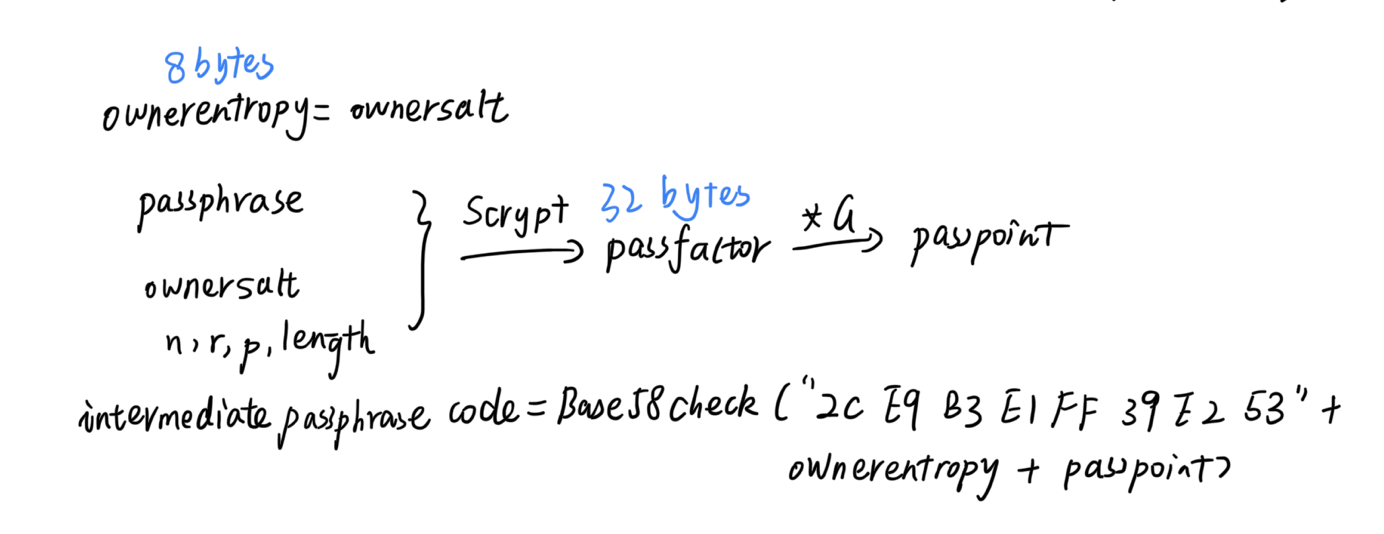
\includegraphics[width=.7\textwidth]{./im-code2.png}
\caption{不使用批号和序列号时方法二的初始化过程}\label{fig-m2initnolnsn}
\end{figure}

 不使用批号和序列号时的初始化过程相对简单. 
 首先生成8字节的随机数$ownersalt$而不是Algorithm~\ref{algo-m2initwithlnsn}~中的4个字节.
 略过批号和序列号字段,此时$ownerentropy$是$ownersalt$的别名.
 Algorithm~\ref{algo-m2initwithlnsn}~中的第4步从$prefactor$生成$passfactor$的计算也略过,
 Scrypt的输出直接作为$passfactor$. 
 \textsf{Base58CheckEncode}编码时使用魔数``2C E9 B3 E1 FF 39 E2 53" (最后一个字节从$0x53$变成$0x51$).
 参见Figure~\ref{fig-m2initnolnsn}.
 
%\begin{algorithm}[h]\footnotesize
%\caption{Initialize without lot sequence}
%  	\begin{algorithmic}[1]
%	    \STATE ownersalt is 8 random bytes instead of 4, and lotsequence is omitted. ownerentropy becomes an alias for ownersalt. 
%		\STATE The SHA256 conversion of prefactor to passfactor is omitted. Instead, the output of scrypt is used directly as passfactor.
%		\STATE The magic bytes are "2C E9 B3 E1 FF 39 E2 53" instead (the last byte is 0x53 instead of 0x51). 
%    \end{algorithmic}
%\end{algorithm}

\subsubsection{加密私钥计算}
第三方拿到中间口令码之后,可以用它为用户生成新的加密私钥.
确切地说,第三方可以为用户生成新的公钥,并将计算对应私钥的所需的信息加密后一并发送给用户,
同时拥有口令和密文信息的人才能从中计算出对应的私钥.  

计算时首先需要设置\textit{flagbyte}, 如果采用压缩形式的公钥派生Bitcoin地址,则设置$flagbyte_5=1$.
如果字段$ownerentropy$中包含批号系列号字段,则设置$flagbyte_6=1$.[\red{todo完善flagbyte设置信息}].
然后生成24个字节的随机数$seedb$,并计算$factorb=\textsf{SHA256}(\textsf{SHA256}(seedb))$.
计算$generatedpubkey = factorb * passpoint$并计算对应的Bitcoin地址
$generatedaddress=\textsf{RIPEMD160}(\textsf{SHA256}(generatedpubkey))[0,\cdots,19]$,
可使用未压缩或者压缩形式的公钥表示,这就是第三方为用户新生成的Bitcoin地址.


%\begin{algorithm}[h]\footnotesize
%\caption{New Public Key Generation}
%  	\begin{algorithmic}[1]
%	    \STATE Set flagbyte.
%	    \STATE Turn on bit 0x20 if the Bitcoin address will be formed 
%	    by hashing the compressed public key (optional). Turn on bit 0x04 
%	    if ownerentropy contains a value for lotsequence.   
%		\STATE Generate 24 random bytes, call this seedb. 
%		Take $SHA256(SHA256(seedb))$ to yield 32 bytes, call this factorb.
%		\STATE ECMultiply passpoint by factorb. Use the resulting EC point 
%		as a public key and hash it into a Bitcoin address using either 
%		compressed or uncompressed public key methodology. 
%		This is the generated Bitcoin address, call it generatedaddress. 
%    \end{algorithmic}
%\end{algorithm}

前述过程完成了新公钥的生成,下面介绍具体的加密过程,
加密过程与方法一中的加密过程类似:
利用Scrypt派生AES的加密密钥,然后对与新公钥关联的$seedb$进行加密.
具体过程在Algorithm~\ref{algo-m2enc}~中给出.

\begin{algorithm}[h]\footnotesize
\caption{使用EC乘法的方法二的加密过程}\label{algo-m2enc}
  	\begin{algorithmic}[1]
	   	\STATE 计算$addresshash=\textsf{SHA256}(\textsf{SHA256}(generatedaddress))[0,1,2,3]$ 
	    	\STATE 用Scrypt从$passpoint$派生32字节值$v=v_1||v_2, v_1 = v[0,\dots, 31], v_2= [32,\dots,63]$
	    	\STATE 计算$ek_1 = \textsf{AES256Encrypt}(block = (seedb[0,\dots,15] \oplus v_1[0,\dots,15]), key = v_2)$
		\STATE 计算$ek_2 = \textsf{AES256Encrypt}(block = ((ek_1[8,\dots,15] || seedb[16,\dots,23])  \oplus v_1[16,\dots,31]), key = v_2)$
		\STATE 密文为$0x01 || 0x43 || flagbyte || addresshash || ownerentropy ||  ek_1[0...7] || ek_2$的 \textsf{Base58CheckEncode}
    \end{algorithmic}
\end{algorithm}

第2步中函数Scrypt的参数passphrase为用户提供的33字节的$passpoint$, 
参数salt为$addresshash || ownerentropy$, $n=1024, r=1, p=1, length=64$.
这里最终数据的格式略有些奇怪,推测是为了方法一中的结果保持长度一致(都是39个字节).
相比较,这里比前面多了一个8字节的$ownerentropy$字段,
\red{因此选取的$seedb$长度也就限制在了24字节 这句怎么理解 跟上一句串不起来},参见Figure~\ref{fig-m2enc}.

%\begin{algorithm}[h]\footnotesize
%\caption{Encryption}
%  	\begin{algorithmic}[1]
%	    \STATE Take the first four bytes of SHA256(SHA256(generatedaddress)) 
%	    and call it addresshas
%	    \STATE Now we will encrypt seedb. Derive a second key from passpoint 
%	    using scrypt 
%		\STATE Parameters: passphrase is passpoint provided from the first 
%		party (expressed in binary as 33 bytes). 
%		salt is addresshash + ownerentropy, $n=1024, r=1, p=1, length=64$. 
%		The "+" operator is concatenation.
%		\STATE Split the result into two 32-byte halves and call them derivedhalf1 
%		and derivedhalf2.
%		\STATE Do $AES256Encrypt(block = (seedb[0...15] \oplus derivedhalf1[0...15]), 
%		key = derivedhalf2)$, call the 16-byte result encryptedpart1
%		\STATE Do $AES256Encrypt(block = ((encryptedpart1[8...15] + seedb[16...23]) 
%		\oplus derivedhalf1[16...31]), key = derivedhalf2)$, call the 16-byte result 
%		encryptedpart2. The "+" operator is concatenation.
%		\STATE The encrypted private key is the Base58Check-encoded concatenation of 
%		the following, which totals 39 bytes without Base58 checksum: 
%		$$0x01 0x43 + flagbyte + addresshash + ownerentropy +  encryptedpart1[0...7] + 
%		encryptedpart2$$
%    \end{algorithmic}
%\end{algorithm}



\begin{figure}[h]
\centering
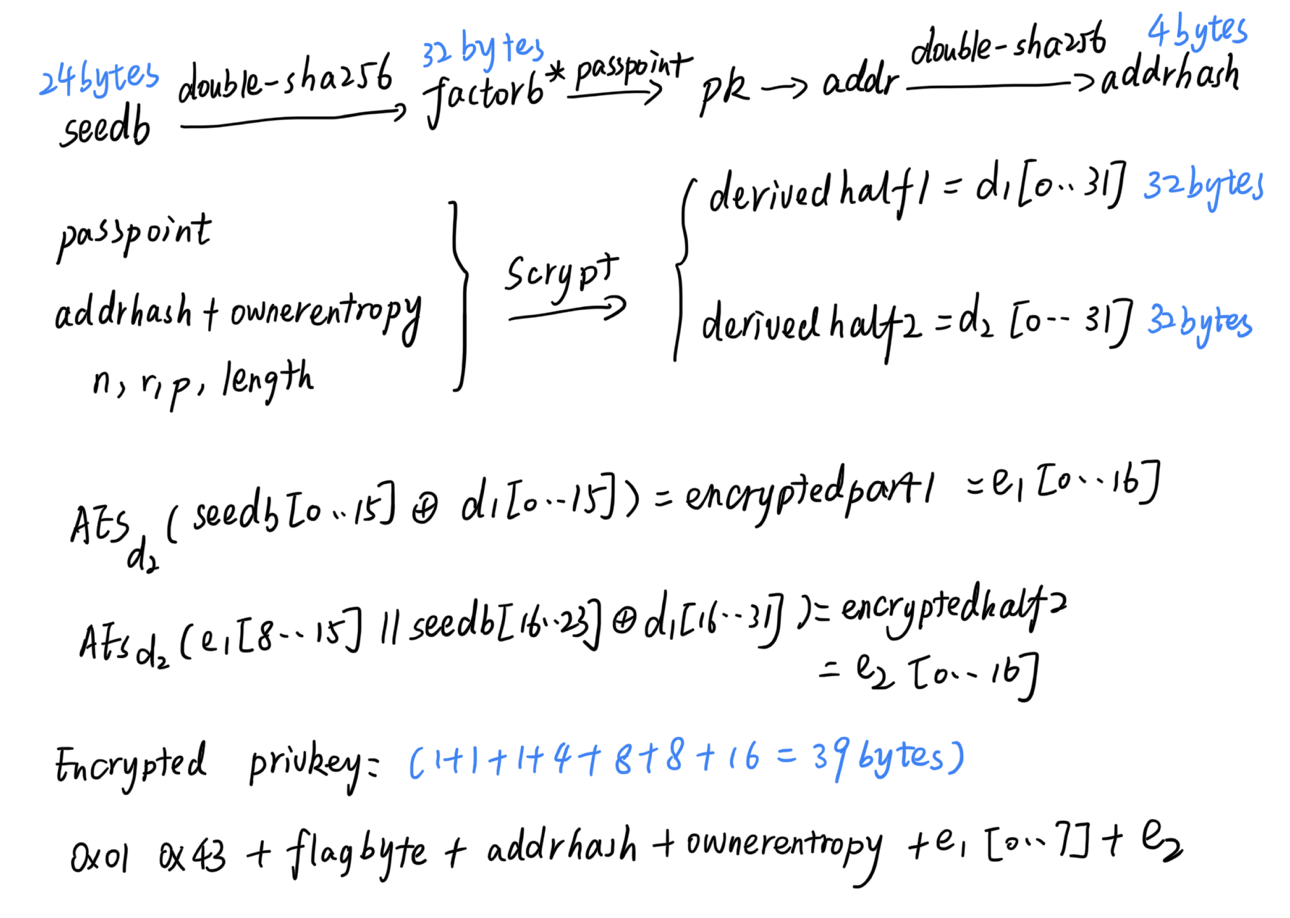
\includegraphics[width=.7\textwidth]{./ec.png}
\caption{使用EC乘法的方法二的加密过程}\label{fig-m2enc}
\end{figure}

\subsubsection{计算新地址对应的私钥}
根据第三方返回的密文计算新私钥的过程在Algorithm~\ref{algo-m2dec}~中展示.
由于新公钥为$passpoint\cdot factorb=passfactor\cdot factorb *G$,
对应的私钥即为$passfactor\cdot factorb$.

\begin{algorithm}[h]\footnotesize
\caption{使用EC乘法的方法二的解密过程与私钥计算}\label{algo-m2dec}
  	\begin{algorithmic}[1]
	   \STATE  用Scrypt函数从$ownersalt$和口令派生$passfactor$并重新计算$passpoint$
	   \STATE 用Scrypt函数从$passpoint, addresshash, ownerentropy$派生$seedb$的解密密钥
		\STATE 用\textsf{AES256Decrypt}解密$ek_2$得到$seedb[16,\dots,23]$和$ek_1[8,\dots,15]$
		\STATE 用\textsf{AES256Decrypt}解密$ek_1$得到$seedb[0,\dots,15]$
		\STATE 用$seedb$计算$factorb$
		\STATE 计算地址$generatedaddress$对应的私钥为$passfactor \cdot factorb$
		\STATE 根据$flagbyte$中的公钥表示形式,从私钥计算对应的Bitcoin地址
		\STATE 根据Bitcoin地址计算$addresshash$并与密文中的字段比较.若不匹配,则口令错误
    \end{algorithmic}
\end{algorithm}

在恢复了新私钥后,客户端还需要验证计算出的私钥与之前$addresshash$给出的地址是否对应,
如果不是,则需要向用户返回错误信息,即用户输入了错误的passphrase.
由于该协议描述的目的场景是针对纸钱包,所以可假定上述编码后的密文的完整性是保证的.
使用EC乘法的加解密过程示例在Listing~\ref{lst-m2}中给出,执行结果在Listing~\ref{lst-m2res}中给出.
%\begin{algorithm}[h]\footnotesize
%\caption{使用EC乘法的方法二的解密过程与私钥计算}\label{algo-m2dec}
%  	\begin{algorithmic}[1]
%	   \STATE  Collect encrypted private key and passphrase from user.
%	   \STATE  Derive passfactor using scrypt with ownersalt and the user's 
%	   passphrase and use it to recompute passpoint
%	   \STATE Derive decryption key for seedb using scrypt with passpoint, 
%	   addresshash, and ownerentropy
%		\STATE Decrypt encryptedpart2 using AES256Decrypt to yield the last 
%		8 bytes of seedb and the last 8 bytes of encryptedpart1.
%		\STATE Decrypt encryptedpart1 to yield the remainder of seedb.
%		\STATE Use seedb to compute factorb.
%		\STATE Multiply passfactor by factorb mod N to yield the private key 
%		associated with generatedaddress.
%		\STATE C\STATE onvert that private key into a Bitcoin address, honoring 
%		the compression preference specified in the encrypted key.
%		\STATE Hash the Bitcoin address, and verify that addresshash from the 
%		encrypted private key record matches the hash. If not, report that the 
%		passphrase entry was incorrect.
%    \end{algorithmic}
%\end{algorithm}


\begin{lstlisting}[language=python, caption = 使用EC乘法的加解密过程示例, label=lst-m2]
def init_enc_with_ec_multi(passphrase,ownersalt,lotsequence):
	if len(ownersalt+lotsequence)!=8:
		assert("ownerentropy must be 8 bytes!")
	# derive prefactor from scrypt
	prefactor=scrypt.hash(passphrase,ownersalt,SCRYPT_N,SCRYPT_R,SCRYPT_P,32)
	#derive passpoint & pack intermediate passphrase code
	if len(lotsequence)==0:
		intermediate_passphrase_code=b'\x2C\xE9\xB3\xE1\xFF\x39\xE2\x53'
		intermediate_passphrase_code+=ownersalt
		passfactor=prefactor
		print("ownersalt",ownersalt)
	else:
		intermediate_passphrase_code=b'\x2C\xE9\xB3\xE1\xFF\x39\xE2\x51'+ownersalt+lotsequence
		prefactor+=(ownersalt+lotsequence)
		passfactor=hashlib.sha256(prefactor).digest()
		passfactor=hashlib.sha256(passfactor).digest()
	k=Key(bytes(passfactor))
	passpoint=k.public_compressed_byte
	intermediate_passphrase_code+=passpoint
	return b58check(intermediate_passphrase_code)

def enc_with_ec_multi(intermediate_passphrase_code,flag_lotseq,flag_compr):	
	#unpack intermediate passphrase code
	intermediate_passphrase_code=base58check.b58decode(intermediate_passphrase_code)
	ownerentropy=intermediate_passphrase_code[8:16]
	passpoint=intermediate_passphrase_code[16:49]

	# generate random seedb to derive new public key & address
	seedb=secrets.token_bytes(24)
	factorb=hashlib.sha256(seedb).digest()
	factorb=hashlib.sha256(factorb).digest()
	k=Key(bytes(passpoint))
	(x,y)=k.public_point()
	c=ecdsa.ellipticcurve.CurveFp(SECP256k1.curve.p(),SECP256k1.curve.a(),SECP256k1.curve.b())
	p=ecdsa.ellipticcurve.Point(c,x,y)
	new_point=p.__mul__(string_to_int(factorb))
	k=Key(new_point.x()+new_point.y())
	addr=k.address() if flag_compr==1 else k.address_uncompressed()
	addrhash=hashlib.sha256(base58check.b58decode(addr)).digest()
	addrhash=hashlib.sha256(addrhash).digest()
	addrhash=addrhash[:4]

	# derive encryption key and use AES to encrypt seedb
	salt=addrhash[:4]+ownerentropy
	d=scrypt.hash(passpoint,salt,1024,1,1,64)
	derivedhalf1=d[:32]
	derivedhalf2=d[32:64]
	m1=[a^b for a,b in zip(seedb[:16],derivedhalf1[:16])]
	e1=AES.new(derivedhalf2).encrypt(bytes(m1))
	m2=[a^b for a,b in zip(e1[8:16]+seedb[16:24],derivedhalf1[16:32])]
	e2=AES.new(derivedhalf2).encrypt(bytes(m2))

	# put all together and encode with base58check
	flagbyte=(0x04 if flag_lotseq==1 else 0)^(0x20 if flag_compr==1 else 0)
	flagbyte=b'\x00' if flagbyte==0 else bytes([flagbyte])
	res=b'\x01\x43'+flagbyte+addrhash[:4]+ownerentropy+e1[:8]+e2

	return b58check(res)

def dec_with_ec_multi(passphrase,enc_priv):
	#unpack encrpted private key
	enc_priv=base58check.b58decode(enc_priv)
	flagbyte=enc_priv[2]
	addrhash=enc_priv[3:7]
	ownerentropy=enc_priv[7:15]
	ownersalt=ownerentropy[:4] if flagbyte&0x04!=0 else ownerentropy
		
	# derive passpoint from passphrase
	prefactor=scrypt.hash(passphrase,ownersalt,SCRYPT_N,SCRYPT_R,SCRYPT_P,32)
	if (flagbyte&0x04==0):
		passfactor=prefactor
	else:			
		prefactor+=ownerentropy
		passfactor=hashlib.sha256(prefactor).digest()
		passfactor=hashlib.sha256(passfactor).digest()
	k=Key(bytes(passfactor))
	passpoint=k.public_compressed_byte

	# derive encryption key for AES from passpoint and decrypt
	d=scrypt.hash(passpoint,addrhash+ownerentropy,1024,1,1,64)
	derivedhalf1=d[:32]
	derivedhalf2=d[32:64]
	m2=AES.new(derivedhalf2).decrypt(enc_priv[23:39])
	seedb2=bytes([a^b for a,b in zip(m2,derivedhalf1[16:32])])
	m1=AES.new(derivedhalf2).decrypt(enc_priv[15:23]+seedb2[:8])
	seedb1=bytes([a^b for a,b in zip(m1,derivedhalf1[0:16])])
	seedb=seedb1+seedb2[8:16]

	#derive private key and verifiy validness of it
	factorb=hashlib.sha256(seedb).digest()
	factorb=hashlib.sha256(factorb).digest()
	k=Key(factorb)
	(x,y)=k.public_point()
	c=ecdsa.ellipticcurve.CurveFp(SECP256k1.curve.p(),SECP256k1.curve.a(),SECP256k1.curve.b())
	p=ecdsa.ellipticcurve.Point(c,x,y)
	new_point=p.__mul__(string_to_int(passfactor))
	k=Key(new_point.x()+new_point.y())
	addrhash_v=k.address() if flagbyte&0x20==1 else k.address_uncompressed()
	addrhash_v=hashlib.sha256(base58check.b58decode(addrhash_v)).digest()
	addrhash_v=hashlib.sha256(addrhash_v).digest()
	if addrhash_v[:4]==addrhash:
		return k.wif()
	else:
		assert("privkey is invalid")
\end{lstlisting}


\begin{lstlisting}[language=bash, caption = Listing~\ref{lst-m2}~的执行结果示例, label=lst-m2res]
Intialization:
Passphrase :  b'passphraseaB8feaLQDENqCgr4gKZpmf4VoaT6qdjJNJiv7fsKvjqavcJxvuR1hy25aTu5sX'
Entropy : b'O\xcaZ\x97@@\xf0\x01'
Intermediate_passphrase_code is  b'passphraseaB8feaLQDENqCgr4gKZpmf4VoaT6qdjJNJiv7fsKvjqavcJxvuR1hy25aTu5sX'

Encryption:
Under this intermediate_passphrase_code, encrypted key is :
b'6PgKDE6dzgJ3cM1Z2fwdhxGyH3W59H1kZjCDHuETevCjCWDh6H7j95X6EF'

Decryption:
Decrypted key plaintext is:
L41y9jwBDLa1h2nHxNnhKGCtn7MDEpMNNvrd1o3WTuoXN8srsrD9
\end{lstlisting}

\subsubsection{新地址的确认码机制}

在第三方为用户生成新的Bitcoin地址之后,用户可能并不需要立即进行解密,
私钥只有在花费对应地址的UTXO时才需要.
但用户需要对产生的新地址进行确认,以防止出现自己无法计算新的地址对应的私钥.
因此,对于使用EC乘法的私钥加密方式,协议还设计了一个独立的验证方式:
第三方可以向用户返回一个以“cfrm38”开头的75个字符的确认码(Confirmation Code),
用来协助用户验证新地址对应的私钥是用户可计算出来的.
 
Confirmation code生成过程如下:

\begin{algorithm}[h]\footnotesize
\caption{确认码生成过程}\label{algo-ccgen}
  	\begin{algorithmic}[1]
	   	\STATE 需要Algorithm~\ref{algo-m2enc}~加密过程中的值:$flagbyte, ownerentropy, factorb, v_1, v_2$
		\STATE 计算$pointb = factorb * G$, 压缩形式表示为33个字节,第一个字节为$0x02$或者$0x03$
		\STATE 计算$pointbprefix = pointb[0] \oplus (v_2[31] \& 0x01)$
		 The first byte is 0x02 or 0x03. XOR it by (derivedhalf2[31] \& 0x01), call the resulting byte pointbprefix.
		\STATE 计算$pointbx_1 = \textsf{AES256Encrypt}(block = (pointb[1...16] \oplus v_1[0...15]), key = v_2)$ 
		\STATE 计算$pointbx_2=\textsf{AES256Encrypt}(block = (pointb[17...32] \oplus v_1[16...31]),key = v_2)$
		\STATE 连接几个值得到33字节$epb = pointbprefix || pointbx1 || pointbx2$
		\STATE 确认码为\small{$\text{ 643BF6A89A} || flagbyte || addresshash || ownerentropy || epb$}的\textsf{Base58CheckEncode}
\end{algorithmic}
\end{algorithm}

除了常数部分,确认码与私钥密文数据的不同之处在于$epb$,其中包含了$factor*G$的信息,
允许用户收到确认码后计算出地址,并可以根据$addresshash$进行验证
如果验证通过,用户可以使用该地址进行交易,并且需要花费时可以计算出相应的私钥.

%验证过程如下:
%\begin{algorithm}[h]\footnotesize
%\caption{Confirmation}
%  	\begin{algorithmic}[1]
%	   \STATE Derive passfactor using scrypt with ownerentropy and 
%	   the user's passphrase and use it to recompute passpoint
%		\STATE Derive decryption key for pointb using scrypt with 
%		passpoint, addresshash, and ownerentropy
%		\STATE Decrypt encryptedpointb to yield pointb
%		\STATE ECMultiply pointb by passfactor. Use the resulting 
%		EC point as a public key and hash it into address using either 
%		compressed or  uncompressed public key methodology as specifid in flagbyte.
%    \end{algorithmic}
%\end{algorithm}


\subsubsection{使用EC乘法的私钥加解密机制的安全性分析}

确认码机制存在一个安全隐患:仅仅靠4个字节的$addresshash$来关联确认码和加密后的密钥是不够的.
一个不诚实的第三方可以提供两个不同的$factorb$,
并且满足经过$\textsf{SHA256}(\textsf{SHA256}(\cdot))$计算后前4个字节相同的两个地址.
这时,仅仅验证确认码是不能够保证用户一定能够计算出他所使用的地址的私钥的.
这也就是说,确认码并不能起到所声称的作用.
比如,第三方计算出$seedb_1$以及相应的$factorb_1$,并计算出新私钥对应的地址$addr_1$, 
$addrhash_1=\textsf{SHA256}(\textsf{SHA256}(addr_1))[0,1,2,3]$.
由于$addrhash_1$只有4字节,第三方可以遍历$factorb$的取值,
直到找到满足$addrhash_2=addrhash_1$的$factorb_2$,计算复杂度为$O(2^{16})$.
这时,第三方就可以根据$seedb_1$来计算加密的密钥,根据$factorb_2$来构造确认码.
由于加密的密钥和确认码中的$addrhash$是相同的,
将确认码和加密的密钥发给用户后, 在用户侧确认码可以验证通过,
如果用户使用计算出的$addr_2$来收款将无法花费相应地址中的资产,
因为他无法计算出$addr_2$对应的私钥(用户只知道$factorb_2*G$的值),
他从加密的密钥中计算出来的私钥对应于 $factorb1 * passfactor$,所以$addr_2$中的钱将无法被花费.

在新私钥的生成中,存在一个安全隐患:在同一个中间口令码下,
如果第三方知道了其中一个加密私钥的明文,那么它就可以绕开用户的口令,
得到在当前中间口令码下派生的所有私钥.
 对于中间口令码 $ipc_1$,第三方生成一个随机数$seedb_1$,
 按照方法二计算,生成的新私钥是$k_1=passfactor * factorb_1 \mod n$, 
 $factorb_1=\textsf{SHA256}(\textsf{SHA256}(seedb_1))$. 
 假如第三方知道了该私钥$k_1$,他就可以计算 $passfactor=k1 * factorb1^{-1} \mod n$, 
 因此,在同一个$ipc_1$下的所有私钥都可以被该第三方计算出来.  
这种场景是存在的:如用户委托第三方为自己生成新的加密私钥后,不小心又委托他对该私钥按照方法一
进行加密,恶意的第三方可以通过对比公钥或地址知道到该私钥是它之前按照方法二生成的,
这时它就具备了作恶的条件.


